\begin{frame}
  \frametitle{Research Overview}
  \begin{minipage}{0.5\textwidth}
    How does the ability to determine forensic-relevant spent nuclear fuel
    attributes using machine learning techniques degrade as less information is
    available?
    \vspace*{2cm}
  \end{minipage}%
  \begin{minipage}{0.5\textwidth}
    \begin{figure}
      \centering
      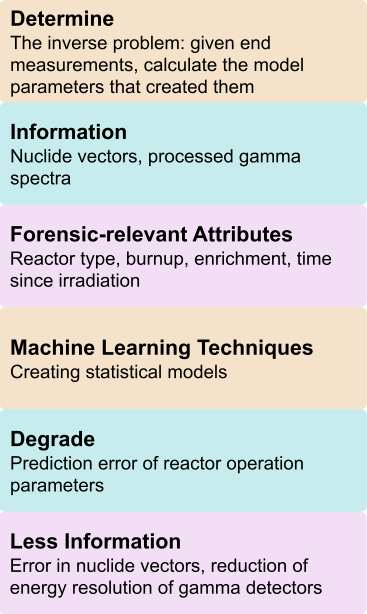
\includegraphics[height=0.75\textheight]{./figures/overview.png}
      \caption{Definitions of terms within the main research question}
    \end{figure}
  \end{minipage}
\end{frame}

\begin{frame}
  \frametitle{Nuclear Security and Forensics}
  \begin{figure}
    \centering
    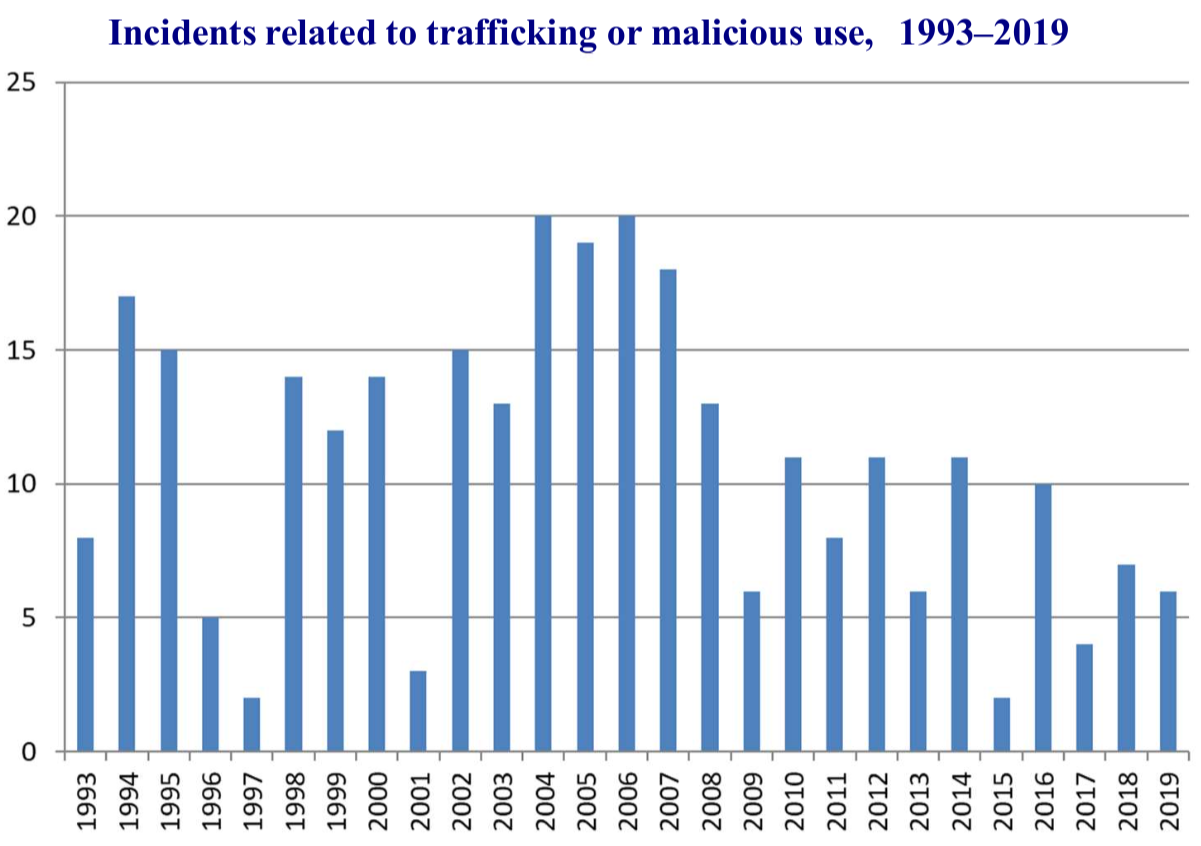
\includegraphics[width=0.8\textwidth]{./figures/nucleartrafficking.png}
    \caption{26 years of incidents related to malicious use: HEU (12), Pu (2), Pu-Be neutron sources (5)\cite{itdb}}
  \end{figure}
\end{frame}

\begin{frame}
  \frametitle{Nuclear Forensics Investigations}
  \begin{adjustwidth}{-10pt}{0pt}
  \begin{minipage}[t]{0.5\textwidth}
    \textbf{Post-detonation}
    \begin{itemize}
      \item Collection: debris, swipe samples
      \item Characterization: rapid analysis of isotope ratios
      \item Goals
      \begin{itemize}
        \item Inverse problem: reconstruct weapon design/yield
        \item Safety: informing disaster response
      \end{itemize}
      \item Data evaluation
    \end{itemize}
  \end{minipage}%
  \hfill
  \begin{minipage}[t]{0.5\textwidth}
    \textbf{Pre-detonation}
    \begin{itemize}
      \item Collection: depends on intercepted material
      \item Characterization: non-destructive and destructive
      \item Goals:
      \begin{itemize}
        \item Inverse problem: material chain of custody
        \item Safety: material handling and security
      \end{itemize}
      \item Data evaluation
    \end{itemize}
  \end{minipage}
  \begin{figure}
    \centering
    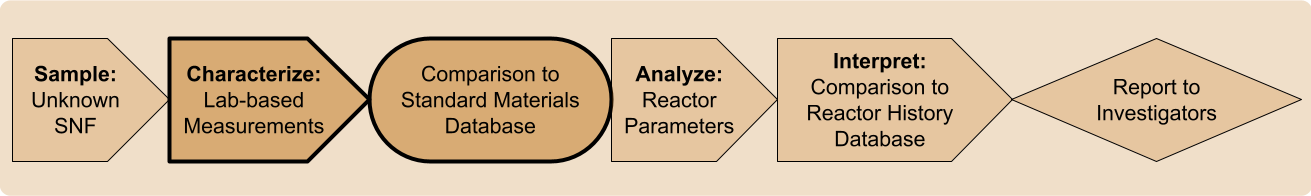
\includegraphics[width=\textwidth]{./figures/forensicsrealworld.png}
    \caption{Typical techincal nuclear forensics workflow}
  \end{figure}
  \end{adjustwidth}
\end{frame}
